
\section{A Customized Programming Environment}
\label{sec:environment}

Beginner programmers are likely to require more guidance and make more mistakes than experienced programmers.
Therefore, we think that is much to gain from a good programming environment which structures the programming experienced and helps the students to identify common mistakes.

% \subsubsection{Visualización y Navegación}
% \begin{itemize}
%   \item syntax highlight
%   \item outline
%   \item hovering
%   \item vista de problems 
%   \item navigate: goto (F3, click), flechita para ir al método que sobrescribe.
%   \item find references 
% \end{itemize}
% 
% \subsubsection{Asistencia}
% \begin{itemize}
%   \item content assist\appendix

\section{Examples of Checks and validations}
\seclabel{ChecksAndValidations}

All the results of the checking and the validation of the program is shown in one integrated view, it is called \emph{Problems}. The figure \figref{problemsview.png} shows a view of this feature. 
There are different types of problems, because these checks and validations are not only used to show type errors or syntax errors, but also to encourage some properties of the program we consider as main topics in the learning process of an OO language.

Here there is a list of all the validations and checking the tool is performing, and a brief reason why they are useful in the teaching of an object oriented language.

Todos los checkeos y problemas
generados se muestran agrupados en una vista dedicada a tal fín (Problems).

% En lo que sigue fui comentando las cosas que ya están dichas pero no quiero borrar esta enumeración porque está muy buena.
\begin{itemize}
   \item \textbf{De sintaxis}: dados por el parser y lexer automáticamente.
  \item \textbf{De estilo}: para promover uniformidad y consistencia de código.
  Ejemplos:
  		\begin{itemize}
  			\item \textit{Nombres}: variables camelcase comenzando en minúscula,
  			nombres de clases camelcase iniciando mayúscula, packages en minúsculas, etc.
  			\item \textit{Orden y agrupamiento}: dentro de un objeto o clase, primero
  			se definen sus referencias internas, luego constructores y finalmente los métodos.
  			\item \textit{Separación de programas}: las clases sólo se pueden definir
  			en archivos de tipo \textit{librería}, no dentro de un \textit{program}.
  			\item \textit{Evitar referencias duplicadas}: no se puede definir una
  			referencia con nombre ya utilizado en alguna otra referencia del contexto (local, método,
  			clase/objeto, etc.). Ni tampoco si ya está definida en la superclase.
		\end{itemize}
  \item \textbf{De resolución de referencias}: para evitar referencias a
  variables inexistentes y, en la medida de lo posible (por ser de tipado
  implícito) de envío de mensajes. Ejemplos:
  		\begin{itemize}
		  \item \textit{Referencias inexistentes}: a variables locales, parámetros, o
		  internas (clase/objeto).
		  \item \textit{Constructores inexistentes}: evaluando existencia de la
		  clase, y compatibilidad en el número de paråmetros.
		  \item \textit{Envío de mensajes (a this)}: al ser a this se pueden realizar
		  checkeos por la existencia del método y compatibilidad de parámetros, incluso sin
		  involucrar al sistema de tipos.
		\end{itemize}
  \item \textbf{De uso de referencias}: para la detección de código
  	erroneo o bien desactualizado. Por ejemplo: warnings por referencias nunca
 	utilizadas, nunca asignadas, o utilización de variables en lugar de valores.
  \item \textbf{De estructura}: evitan por ejemplo inconsistencias en las
  estructuras creadas por el alumno. Por ejemplo, se checkea
  que un método marcado como \textit{override} efectivamente esté
	sobrescribiendo.
  \item \textbf{De tipos}: verifican compatibilidad de referencias en base a sus
  tipos. Por ejemplo ante envío de mensajes, o asignaciones de variables. Basado
  en el sistema de tipos.
\end{itemize}


\section{Implementation}
\label{sec:implementation}
\np{Qué podemos decir de esto}

\section{Images}
Imágenes y otros detalles de wollok que no entran en las 6/7 páginas del artículo

	\begin{figure}[p]
	    \centering
		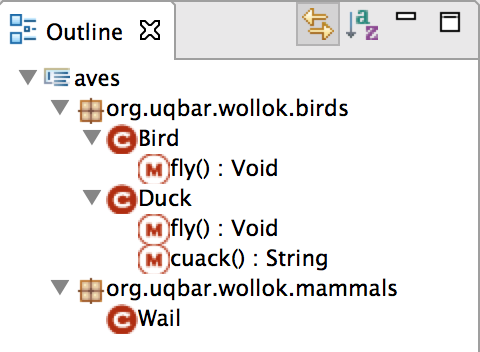
\includegraphics[scale=0.5]{images/wollok-paper-outline.png}
	    \caption{Outline View: muestra un resumen del contenido del archivo}
	    \label{fig:outline.png}
	\end{figure}
	
	\begin{figure}[p]
	    \centering
		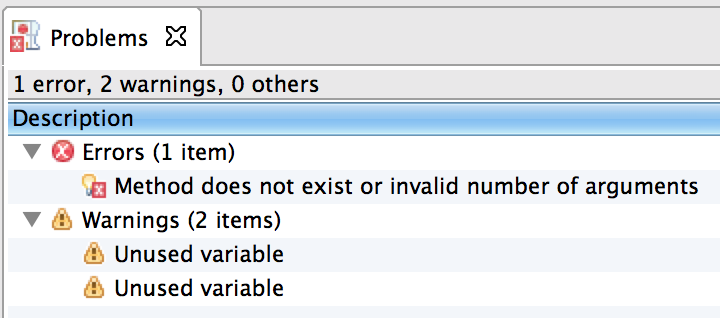
\includegraphics[scale=0.5]{images/wollok-paper-check-problemsview.png}
	    \caption{Vista de Problemas: errores y warnings}
	    \label{fig:problemsview.png}
	\end{figure}
	
	\begin{figure}[p]
	    \centering
		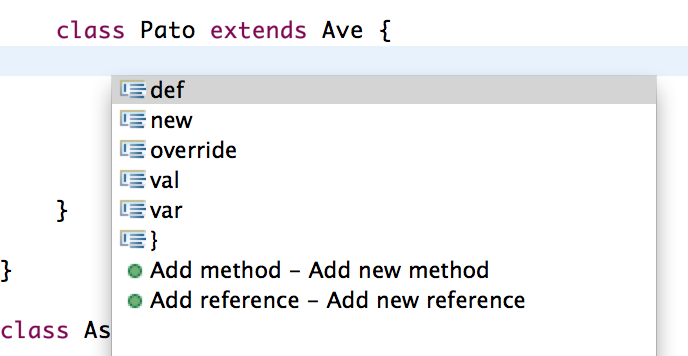
\includegraphics[scale=0.5]{images/wollok-paper-codetemplates.png}
	    \caption{Code Assist: templates para crear código rápidamente}
	    \label{fig:codetemplates.png}
	\end{figure}

	\begin{figure}[p]
	    \centering
		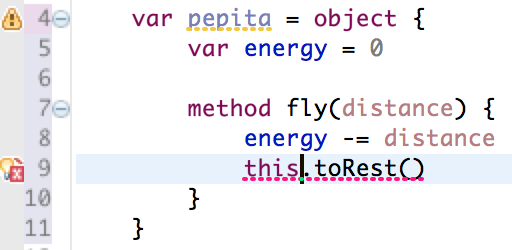
\includegraphics[scale=0.5]{images/wollok-paper-check-noMethodOnThis.png}
	    \caption{Checkeo de método inexistente en this}
	    \label{fig:check-noMethodOnThis.png}
	\end{figure}


\end{document}

%   \item quick fixes
%   \item code templates (nuevo)
% \end{itemize}
The Wollok programming environment includes a lot of features that provide guidance to the student.
\emph{Content assist} shows the students what are his possibilities at any moment and feeds automatically into the code the most usual constructs, 
allowing the student to concentrate less on syntax and more in the modelling of the exercise problem.
\emph{Quick-fixes} allow Wollok not only to highlight problems in the student's code but also to propose automatic solutions for some usual mistakes.
\emph{Advanced code navigation} and \emph{smart reference searches} allow the programmer to better understand the dependencies in his program.
\np{¿Se les ocurre cómo mejorar eso?}
Moreover, \emph{automatic class diagrams} provide a high level view of the program and also helps understanding.

% Detect mistakes
Also, the programming environment has many tools intended to help detecting mistakes, even while the student is writing code.
\emph{Syntax highlighting} helps identify the most simple mistakes by providing immediate feedback when something is not right. 
Moreover, the environment provides \emph{real-time highlights} for syntactic mistakes.
Finally, the \emph{type inferer} allows to detect more subtle mistakes.
All these tools allows the student to gain more control of his code, keeping him away from feeling lost, 
which is otherwise a common situation for a student walking his first steps into programming.

% Este no sé cómo ponerlo, es muy crítica al smalltalk.
% 8-reducir errores frustrantes: se cancela la edicion por tener 1 solo editor de metodo por ves (poder visualizar más que un sólo método simul), evitar errores de imagenes)

\medskip
% Type inferer
The type inferer is one of the most distinctive characteristics of the Wollok programming environment.
We think that type inference is key to a simple programming environment.
On one side, it allows to detect lots of common mistakes \emph{before running the program}:
if an object does understand a message, if a wrong argument is passed, if incompatible types are mixed or even miss-spellings.
In environments without this capability it takes more time to detect errors.
Moreover, it is not uncommon that a type mistake produces a runtime error in a place different from where the mistake was done, producing confusion.

Still, providing a type inferer for a language such as Wollok has many subtleties, which deserves an independent study \cite{type inferer}.
On one side we require it to be able to work without type annotations and at the same time provide feedback useful for an inexperienced programmer.
On the other side, the type system is rather complex;
for example, the presence of stand-alone objects requires the type system to handle \emph{structural types}, since a named type system would not allow them to be treated polymorphically.
Also, we want to be able to treat polymorphically stand alone objects with class-based objects.

\subsubsection{Checks and Validations}

The IDE provides a way of showing some interesting checks and validations. This validations are organized and showed in a common way, using a dedicated section of the user interface for their display. In this way the IDE can be used to teach main concepts, not only showing syntax errors. Some of the errors are described in the \secref{ChecksAndValidations}
